\let\negmedspace\undefined
\let\negthickspace\undefined
\documentclass[journal]{IEEEtran}
\usepackage[a5paper, margin=10mm, onecolumn]{geometry}
%\usepackage{lmodern} % Ensure lmodern is loaded for pdflatex
\usepackage{tfrupee} % Include tfrupee package

\setlength{\headheight}{1cm} % Set the height of the header box
\setlength{\headsep}{0mm}     % Set the distance between the header box and the top of the text

\usepackage{gvv-book}
\usepackage{gvv}
\usepackage{cite}
\usepackage{amsmath,amssymb,amsfonts,amsthm}
\usepackage{algorithmic}
\usepackage{graphicx}
\usepackage{textcomp}
\usepackage{xcolor}
\usepackage{txfonts}
\usepackage{listings}
\usepackage{enumitem}
\usepackage{mathtools}
\usepackage{gensymb}
\usepackage{comment}
\usepackage[breaklinks=true]{hyperref}
\usepackage{tkz-euclide} 
\usepackage{listings}
% \usepackage{gvv}                                        
\def\inputGnumericTable{}                                 
\usepackage[latin1]{inputenc}                                
\usepackage{color}                                            
\usepackage{array}                                            
\usepackage{longtable}                                       
\usepackage{calc}                                             
\usepackage{multirow}                                         
\usepackage{hhline}                                           
\usepackage{ifthen}                                           
\usepackage{lscape}
\usepackage{circuitikz}
\tikzstyle{block} = [rectangle, draw, fill=blue!20, 
    text width=4em, text centered, rounded corners, minimum height=3em]
\tikzstyle{sum} = [draw, fill=blue!10, circle, minimum size=1cm, node distance=1.5cm]
\tikzstyle{input} = [coordinate]
\tikzstyle{output} = [coordinate]


\begin{document}

\bibliographystyle{IEEEtran}
\vspace{3cm}

\title{6.6.4}
\author{EE24BTECH11047 - Niketh Prakash Achanta}
 \maketitle
% \newpage
% \bigskip
{\let\newpage\relax\maketitle}

\renewcommand{\thefigure}{\theenumi}
\renewcommand{\thetable}{\theenumi}
\setlength{\intextsep}{10pt} % Space between text and floats


\numberwithin{equation}{enumi}
\numberwithin{figure}{enumi}
\renewcommand{\thetable}{\theenumi}

\textbf{Question}: Find the equation of the normal to the curve $x^2=4y$ that passes through the point $\brak{1,2}$.\\
\textbf{Solution}
\\
\textbf{Theoretical solution:}\\

The equation of the curve is 
\begin{align}
x^2 = 4y.
\end{align}

\textbf{Step 1: Slope of the tangent}  
Differentiating $\brak{x^2 = 4y}$ with respect to x, we get:
\begin{align}
    2x &= 4 \frac{dy}{dx}, \\
    \frac{dy}{dx} &= \frac{x}{2}.
\end{align}

Thus, the slope of the tangent at a point \((x_1, y_1)\) is:
\begin{align}
\text{slope of tangent} = \frac{x_1}{2}.
\end{align}

\textbf{Step 2: Slope of the normal}  
The slope of the normal, being the negative reciprocal of the slope of the tangent, is:
\begin{align}
\text{slope of normal} = -\frac{2}{x_1}.
\end{align}

\textbf{Step 3: Equation of the normal}  
The equation of the normal passing through $\brak{x_1, y_1}$ is:
\begin{align}
    y - y_1 &= -\frac{2}{x_1}(x - x_1), \\
    x_1y - x_1y_1 &= -2(x - x_1), \\
    x_1y + 2x &= 2x_1 + x_1y_1.
\end{align}

\textbf{Step 4: Using the condition that the normal passes through (1, 2)} \\
Substitute $\brak{x = 1, y = 2}$ into the normal equation:
\begin{align}
    x_1(2) + 2(1) &= 2x_1 + x_1y_1, \\
    2x_1 + 2 &= 2x_1 + x_1\left(\frac{x_1^2}{4}\right), \\
    2 &= \frac{x_1^3}{4}, \\
    x_1^3 &= 8, \\
    x_1 &= 2.
\end{align}

\textbf{Step 5: Finding $y_1$}  
Substitute $x_1 = 2$ into $x_1^2 = 4y_1$ to find $y_1$:
\begin{align}
    (2)^2 &= 4y_1, \\
    y_1 &= 1.
\end{align}

\textbf{Conclusion:}  
The foot of the normal is $\brak{2, 1}$.
\\
\textbf{Computational solution :}\\
\section{Introduction}
This document describes the computation performed in the given C and Python code, which involves generating function values and performing gradient descent optimization.

\section{Point Generation}
The C function computes a set of points $(x, f(x))$ over a specified range. The function follows these steps:
\begin{itemize}
    \item Define an initial value $x_0 = -10$.
    \item Compute the step size as:
    \begin{equation}
        h = \frac{2x_0}{n}
    \end{equation}
    where $n$ is the number of points.
    \item Iteratively update $x$ and compute $f(x) = x^2/4$.
\end{itemize}

\section{Gradient Descent Algorithm}
The C function \textbf{run\_gradient\_descent} implements the gradient descent algorithm to find the minimum of a function $f(a)$. The process involves:
\begin{itemize}
    \item Initializing the guess $a_0$.
    \item Iteratively updating $a$ using the formula:
    \begin{equation}
        a_{n+1} = a_n - \alpha f'(a_n)
    \end{equation}
    where $\alpha$ is the step size.
    \item The process stops when $|f'(a_n)|$ is below a specified tolerance.
\end{itemize}

\section{Python Implementation}
The Python script uses \brak{ctypes} to interface with the compiled C functions. The key components include:
\begin{itemize}
    \item Calling \textbf{generate\_points} to compute function values.
    \item Defining the derivative function:
    \begin{equation}
        f^{\prime}\brak{x_n} = x_n/2
    \end{equation}
    \item Running \textbf{run\_gradient\_descent} to find the minimum of the function.
\end{itemize}

\section{Results and Visualization}
A scatter plot highlights the computed minimum.
\begin{figure}[!ht]
    \centering
    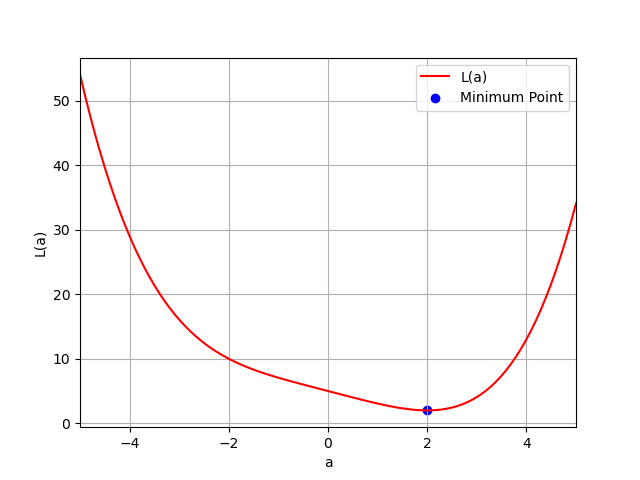
\includegraphics[width=\columnwidth]{/home/niketh/EE1003/Assignment-4/figs/Fig1.png}
    \caption{}
\end{figure}
\end{document}

